\subsection{RQ5:What are the personal expectations and desire reigning in the industry?}
\label{RQ5}
This is the most interesting question. In fact, this question truly answers about the existing condition of our software industry. There are many problems and every one of them has solution. All about these have come into this question beautifully. Every employee has something to tell to their managers. Likewise, every manager has some demands from his subordinates. Not only these, they all have some expectations from government and also universities. All of these expectations are included in the answer of this research question.

\begin{itemize}
    \item Expectation from Managers
    \item Expectation from Employees
    \item Expectation from Potential Candidates
    \item Expectation from Universities
    \item Expectation from Government
    \item Training provide by Companies
\end{itemize}


\subsubsection{Expectation from Managers}
\label{Expectation from Managers}
\begin{figure}[htbp]
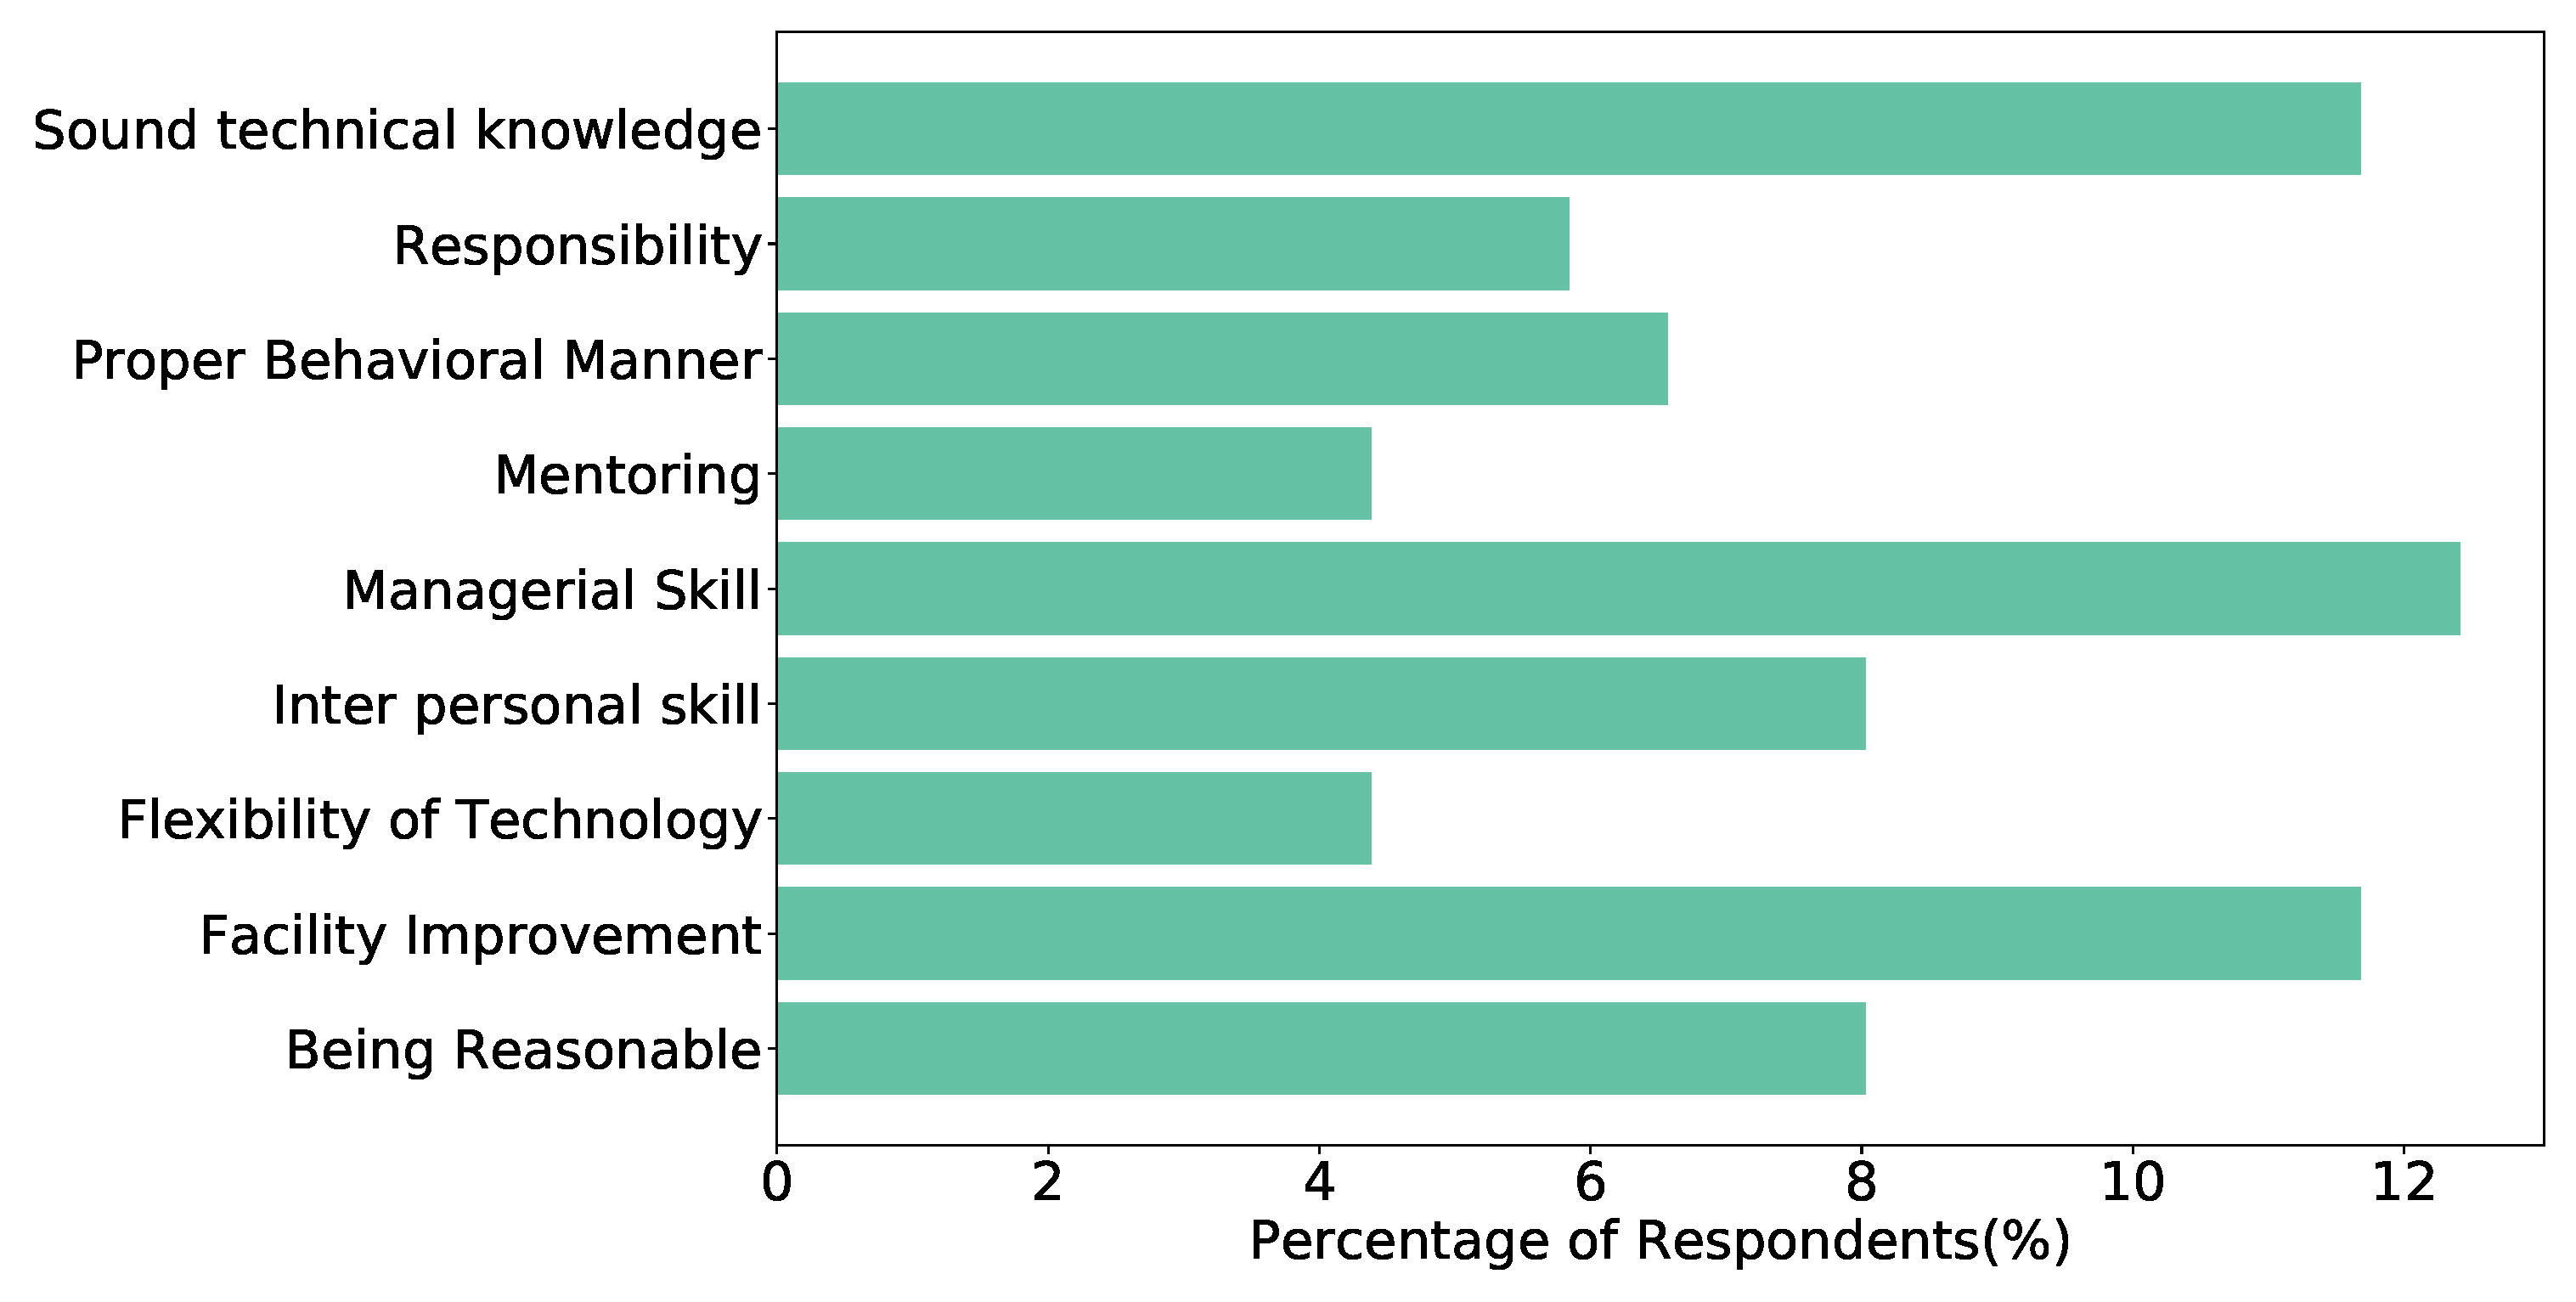
\includegraphics[scale=0.28]{Figures/Managers_Expectation.eps} 
\caption{Respondents expectation from managers}
\label{fig:managers expectation}
\end{figure}

\begin{enumerate}
    \item \textbf{Proper behavioural manner}: 6.57\% respondents expect well behaviour from management. It is clear from survey responses employees hates micro-management the most.
     \surveyquote{Well Behaved and Proper Project Timeline}{28}
    
    
    \item \textbf{Being Reasonable}:  The managers should be reasonable in decision making. In order to get acquainted with the needs and necessities of the employees, managers should have a wide open view towards their desire. About 8.03\% of the respondents have expressed in this way.
    \surveyquote{Give reasonable time for a task and do proper comment on that task}{38}
    
    
    \item \textbf{Flexibility of Technology}: It is very important for the managers to be up-to-date with the latest technology. Managers without a strong background of technical knowledge are really difficult to work with. 4.38\% of total respondents have demanded for a manager with sufficient technical knowledge. 
    \surveyquote{Allow to use latest technologies and good practice to ensure company and their employee are updated with the current world. And also honor according to knowledge and quality works. In the company should have knowledge sharing, training sessions}{48}
    
    
    
    \item \textbf{Responsibility}: Managers should take the responsibility for the works being done. A responsible manager can inspire the employees under him to a great extent. About 5.84\% of the total respondents aspire for a responsible manager to work with.
    \surveyquote{Take responsibility}{82}
    
    
    \item\textbf{Facility Improvement}: 11.68\% respondents mentioned that they look for facility improvements from managers. These facilities include increased remuneration, good working environments, team building events, positive recognition, yearly evaluation etc.
    \surveyquote{Ensuring an environment where positive criticisms regarding code and people can be done.}{57}
    
    
    \item\textbf{Inter Personal Skill}: 8.03\% respondents expects inter personal skills among managers. The skills include proactive, leadership attitude, good communication skill and empathy.
    \surveyquote{Ownership, Proactiveness, Leadership attitude, Good inter-personal and communication skills}{42}
    
    
    \item\textbf{Managerial Skill}: The managers should have solid technical knowledge. He/she must be farsighted. One of the most important part of this post is management of requirements. He should have clear  understanding of required manpower and resources. Respondents marked that timeline management is another managerial skill they expect from managers.
    \surveyquote{1. Strong grasp on the requirements before assigning me to a project 2. Maintain informed and feasible deadlines}{8}
    
    
    \item \textbf{Mentoring}: Respondents also look  a mentor character in manager. They expect direction, advice and opportunity from managers for their career growth.
    \surveyquote{To supervise and to advise to follow specific career plan}{9}
    
    
    \item\textbf{Sound Technical Knowledge}: 11.68\% respondents emphasizes on technical knowledge among managers.
    \surveyquote{Should be technically active}{14}

\end{enumerate}


\subsubsection{Expectation from Employees}
\label{Expectation from Employees}
\begin{figure}[htbp]
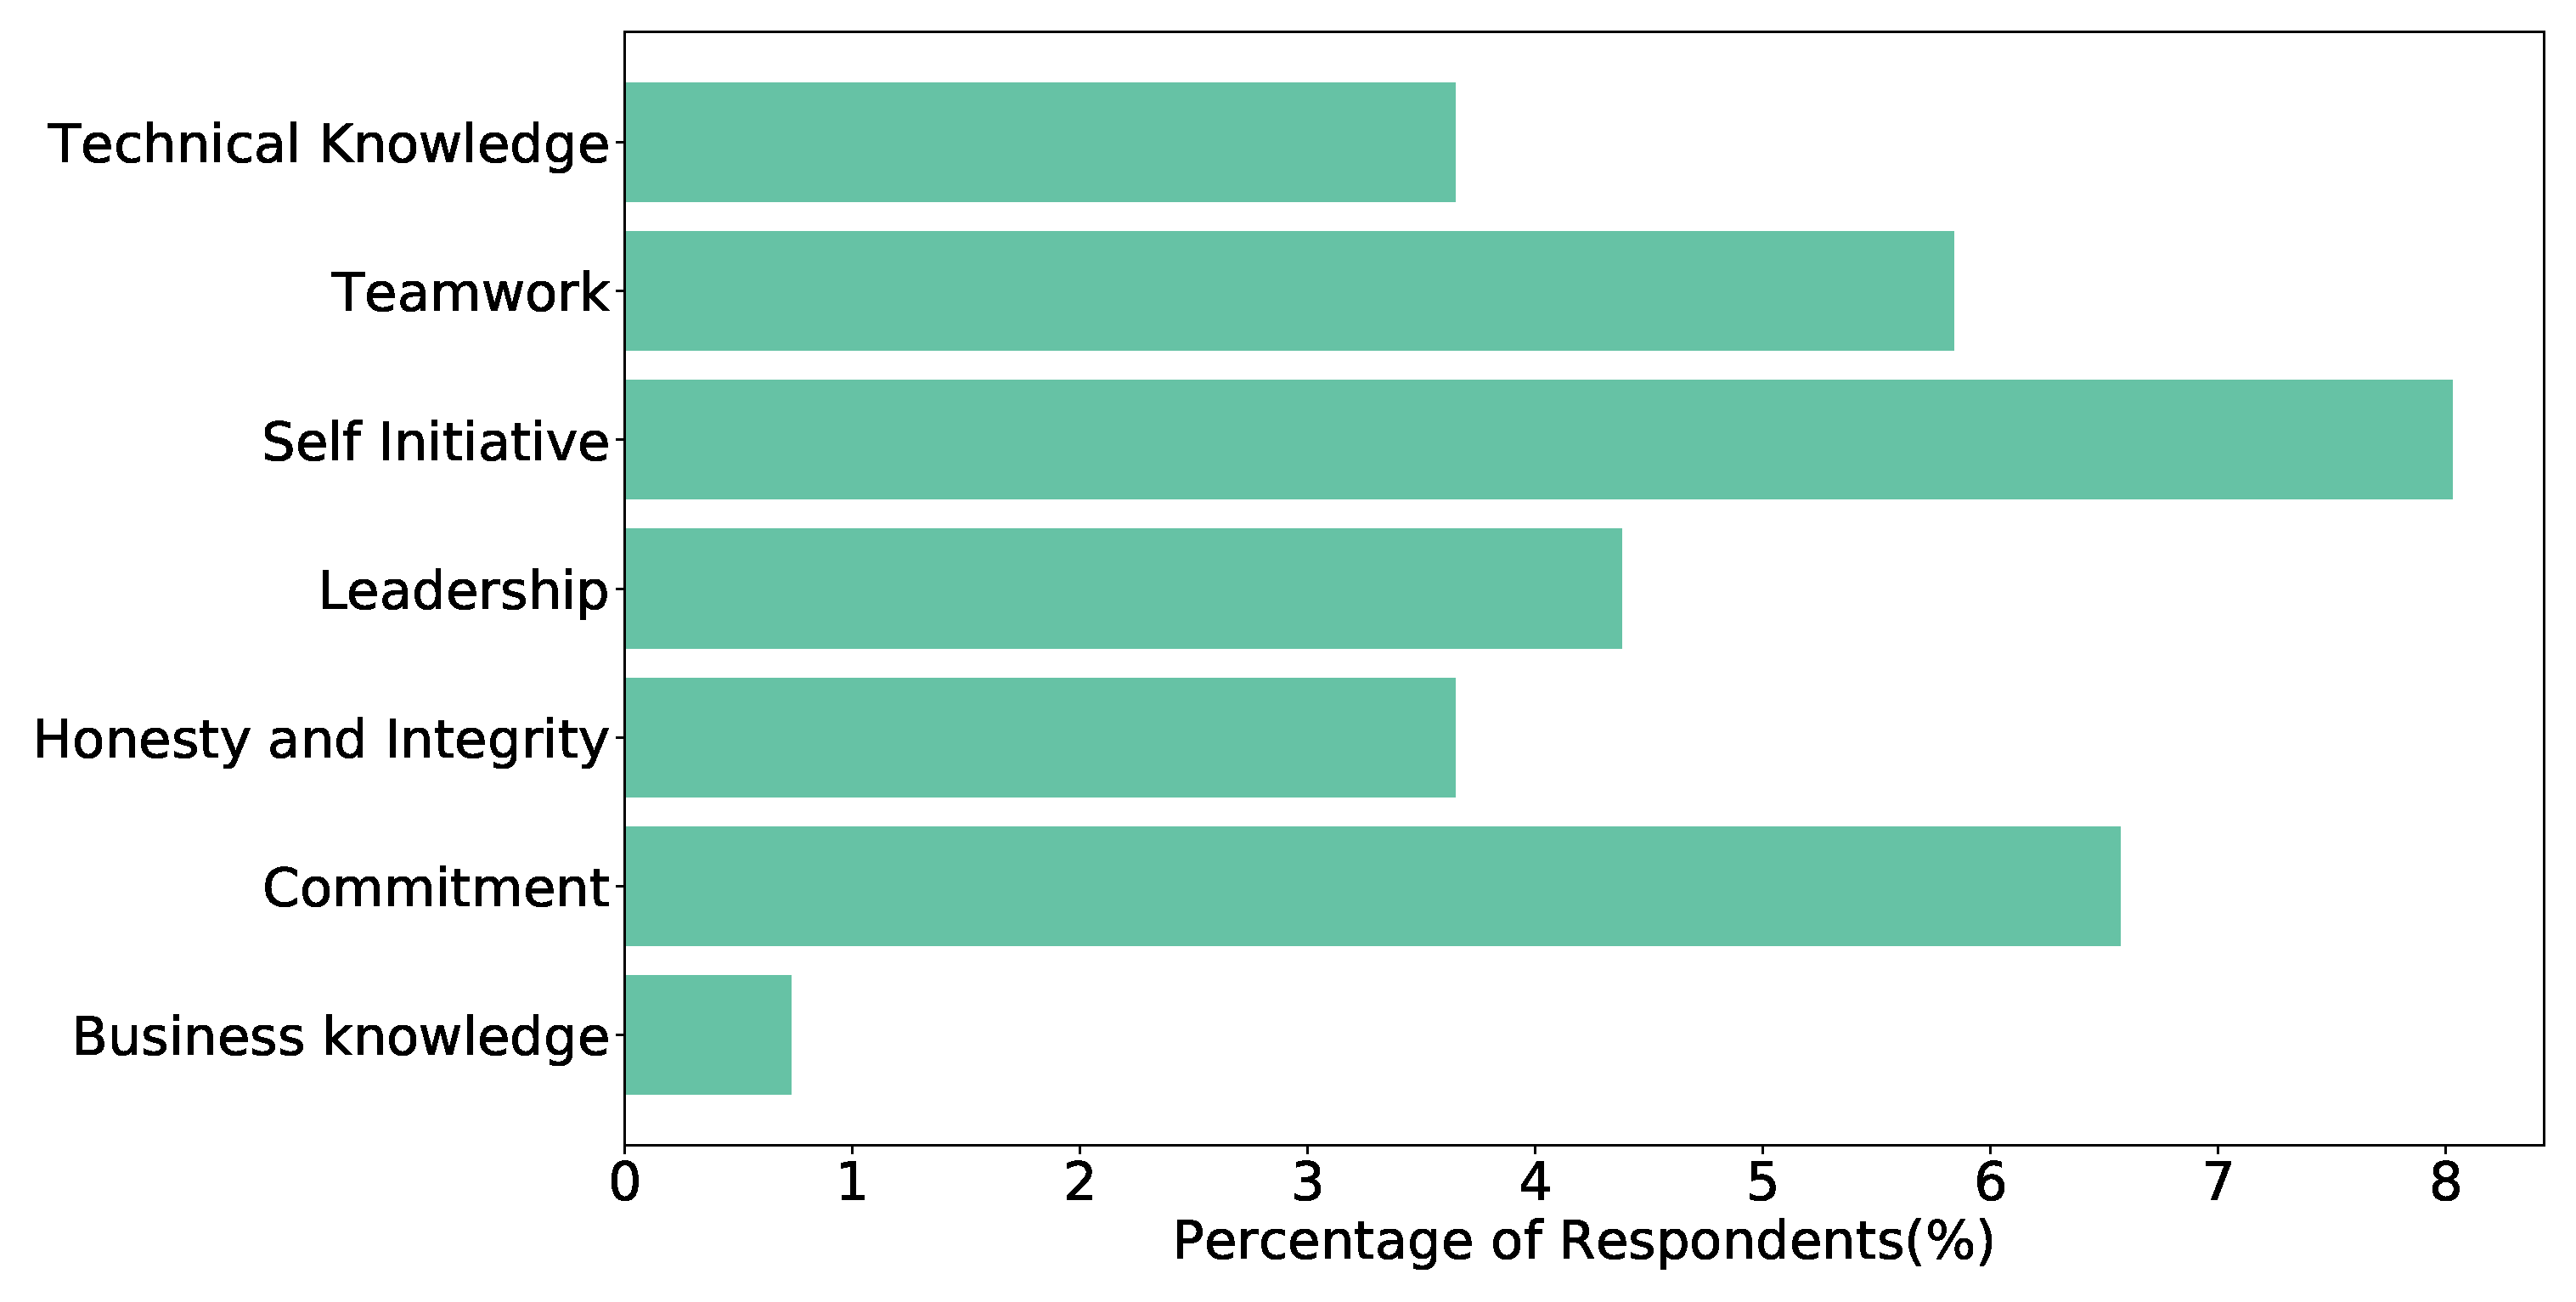
\includegraphics[scale=0.28]{Figures/EmployeeExpectation.eps} 
\caption{Respondents expectation from employees}
\label{fig:employees expectation}
\end{figure}

\begin{enumerate}

    \item \textbf{Technical Knowledge}: 3.65\% respondents look for solid technical knowledge and clean codes from employees.
    \surveyquote{Code in a way that is a delight to read}{49}
    
    
    
    \item \textbf{Teamwork}:It is very obvious to be expected. In a software industry, not a single product is created single-handedly. A bunch of people from various sectors work on the product, and to make a good product, team work between these members is very important. 5.84\% of the managers responded desired this behaviour from the employees.
    \surveyquote{Employees should be cooperative and share knowledge with each other and work together like family member}{51}
    
    
    \item \textbf{Self Initiative}: An employee should learn in his own interest. In industry, everyone is occupied with himself. There is no space to be spoon-fed. A self-initiative worker will find his way even if there are many obstacles.8.03\% people have appraised self-initiative attitude.
    \surveyquote{Clean code which creates less error. Coming up with optimization proposals on features developed earlier. Documentation in a timely manner}{10}


    \item \textbf{Leadership}: 4.38\% respondents look for leadership attitude like ownership of work, proactive and adaptiveness among employees.
    \surveyquote{Sincere, Feel owner ship of project/product and good teamplayer}{107}
    
    \item \textbf{Honesty and Integrity}: Not only coding and academic knowledge, but also behavioural manner plays a great role in deciding about a employee’s career. 3.65\% people want a well behaved and mannered employee to work with.
    \surveyquote{honesty, integrity, self initiative and clear communication}{35}
    
    
    \item \textbf{Commitment}: 6.57\% managers have demanded commitment from their employees. A more committed employee will give better performance than a less committed employee, as he does not give full attention to the job.
    \surveyquote{They will stay for long term and perform up to expectations, learn from mistakes}{114}
    
    
    \item \textbf{Business Knowledge}:  It is important to have knowledge of business domain when designing a solution or dealing with a customer. Thus respondents look for business knowledge like negotiation among employees.
    \surveyquote{Understanding the business, end user and user stories}{82}


\end{enumerate}


\subsubsection{Expectation from Potential Candidates}
\label{Expectation from Potential Candidates}
\begin{figure}[htbp]
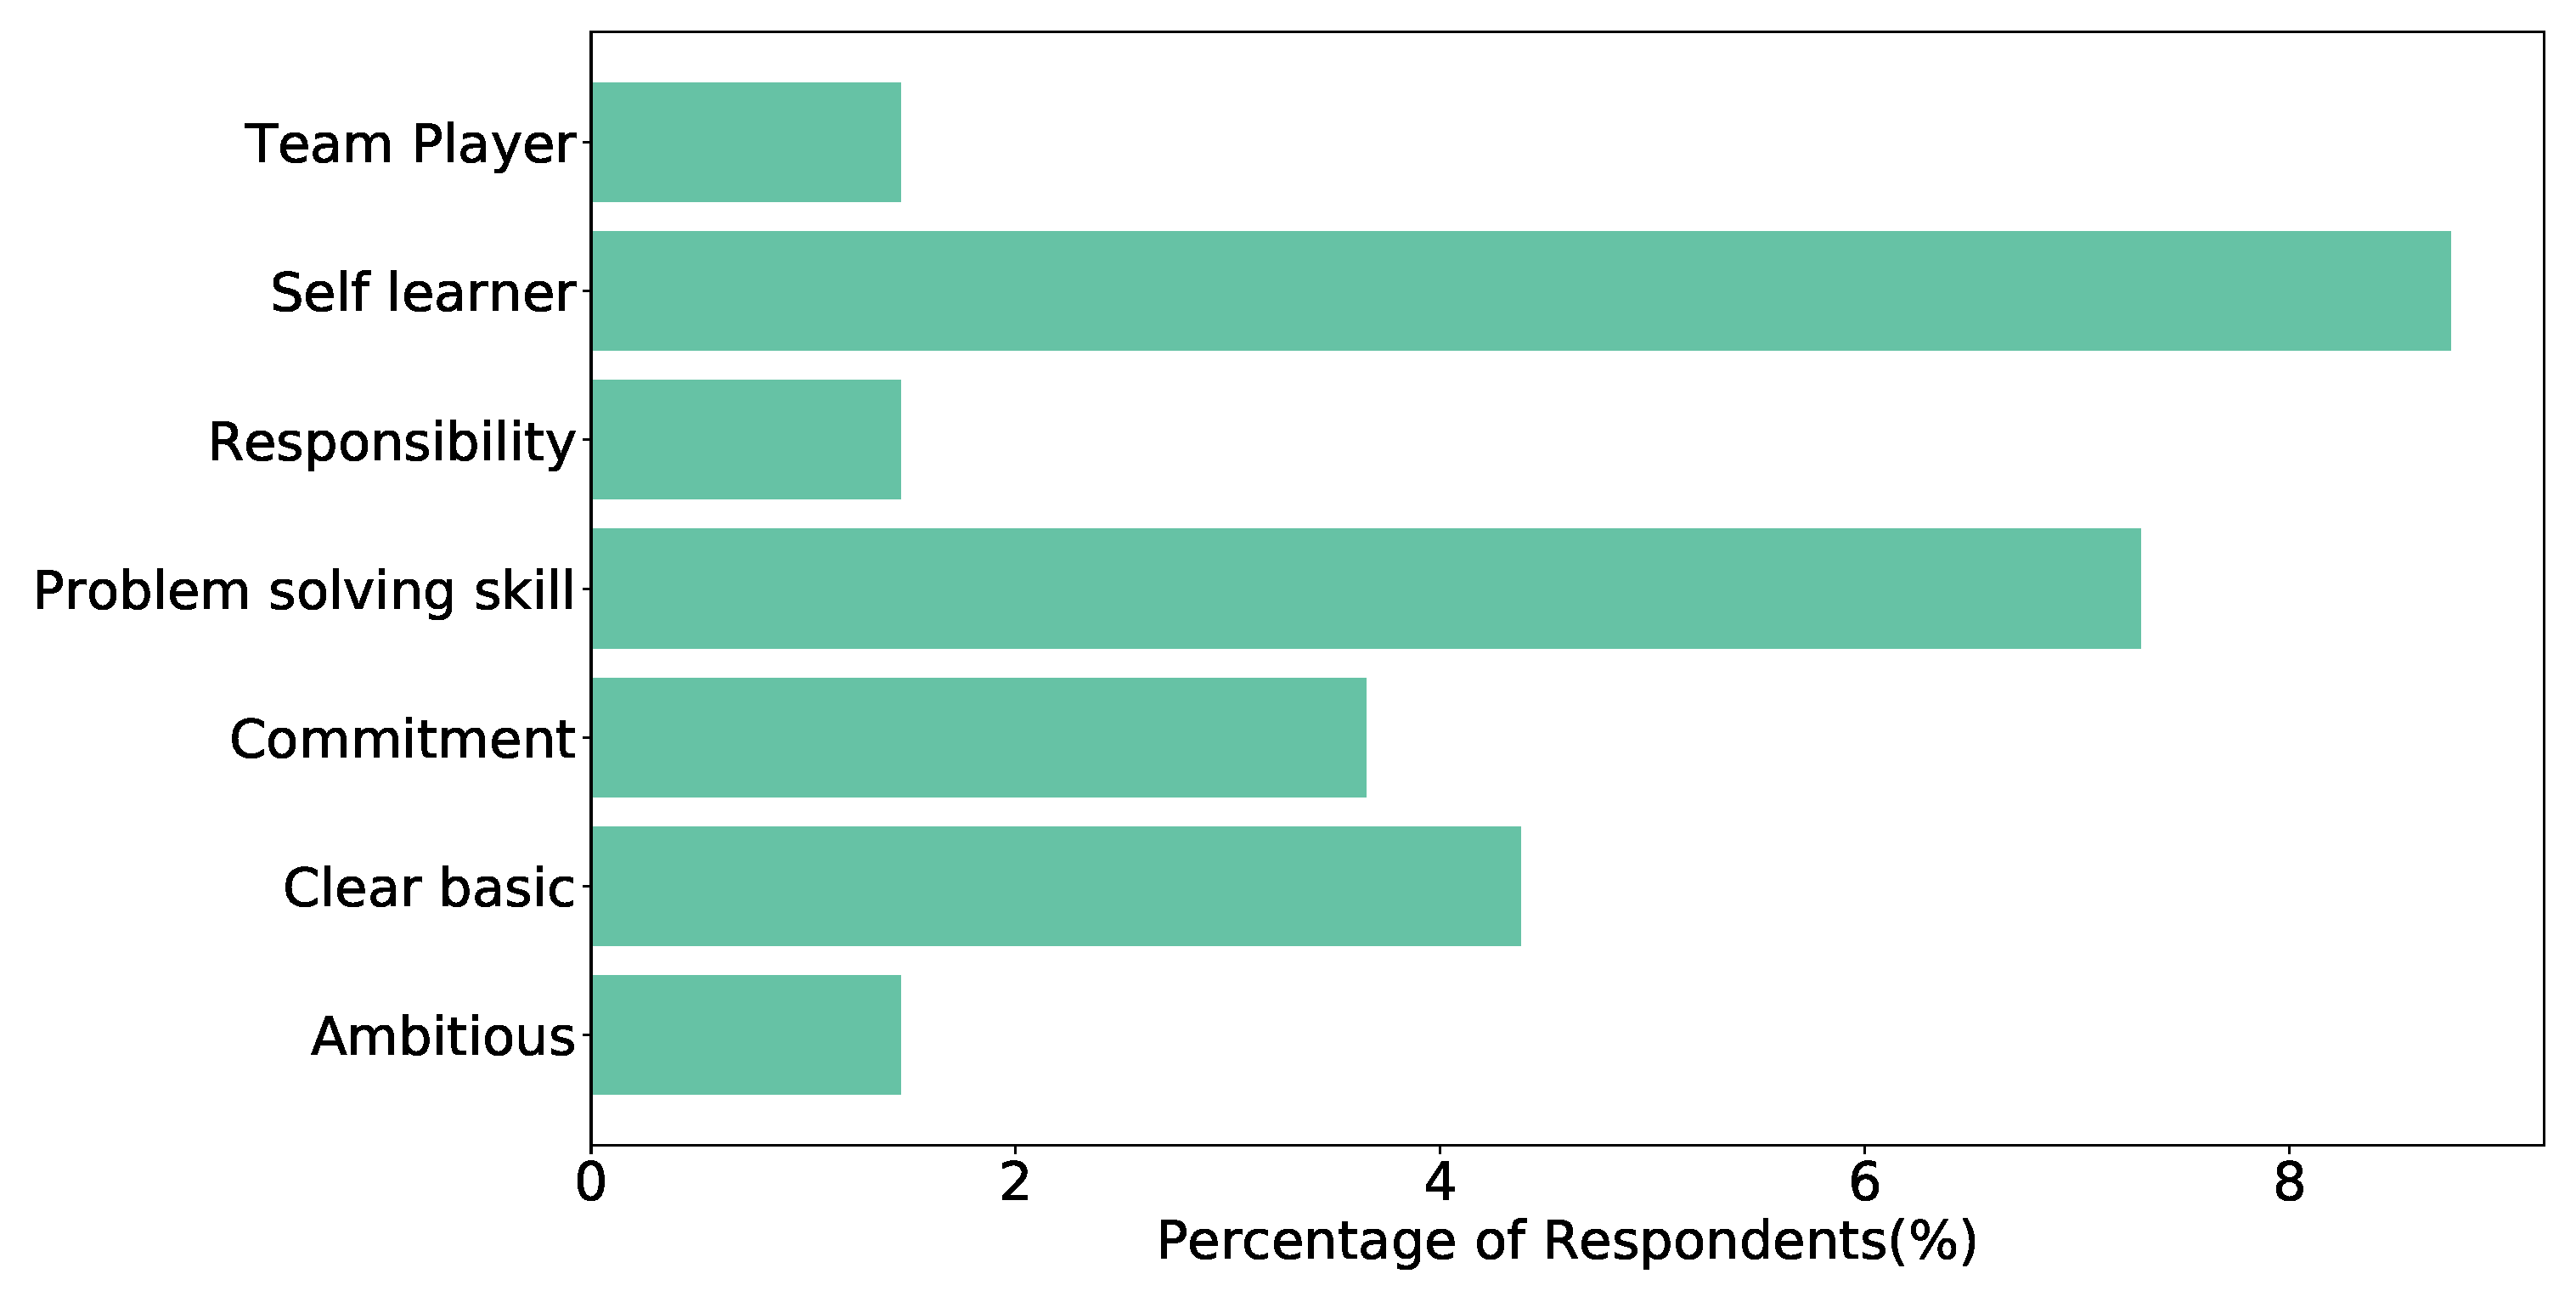
\includegraphics[scale=0.28]{Figures/CandidatesExpectation.eps} 
\caption{Respondents expectation from potential candidates}
\label{fig:candidate expectation}
\end{figure}

\begin{enumerate}
    \item \textbf{Team-player}:Team work plays the most significant role for success in a specific product in any industry. Every potential job candidate should be prepared to work together with a group of people to fulfill the production of a software. 1.46\% wanted to hire a team player than an individual talent.
    \surveyquote{Enthusiastic, Self-learner, Team player}{5}
    
    
    \item\textbf{Self-learner}: Most of the software companies does not have luxury to arrange training or to assign mentor. Thus employers look for self-learning capability among candidates.
    \surveyquote{Self learner, Know well what you know}{53}
    
    \item\textbf{Responsibility}: 1.46\% respondents look for ownership of work or sense of responsibility among potential candidates.
    \surveyquote{taking ownership of responsibility}{66}
    
    
    \item\textbf{Problem-solving Skill}: Problem solving skill distinguishes a potential candidate from others. A candidate with good problem solving capability can adapt to any team. Problem-solving skill is desired by 7.3\% of the total respondents.
    \surveyquote{I am assuming that the potential candidates refer to the freshers in this question. I expect freshers to be very good with problem solving with strong analytical ability. Good university projects are plus}{10}
    
    \item\textbf{Commitment}: 3.65\% of the respondents want commitment from the freshers who are willing to enter into the software industry. He should give his best to attain the goal.
    \surveyquote{Commitment and dedication}{114}
    
    \item \textbf{Clear basic}: Every company want that freshers will have a clear understanding about the basic knowledge. They do not want knowledge about industry, they want clear knowledge about things like programming language, data structures and algorithm. 4.38\% of the respondents want clear basics form the candidates.
    \surveyquote{Professionalism and clear understanding of technologies what they know}{85}
    
    \item\textbf{Ambitious}: 1.46\% respondents prefer ambitious candidates. They look for enthusiasm and hunger for success among candidates.
    \surveyquote{ Knowing what he/she knows and what not, honesty, good problem solving capacities, team-man, absolutely no ego or arrogance, can get things done, ambitious, sincerity, discipline}{42}
\end{enumerate}


\subsubsection{Expectation from University}

\label{Expectation from University}
\begin{figure}[htbp]
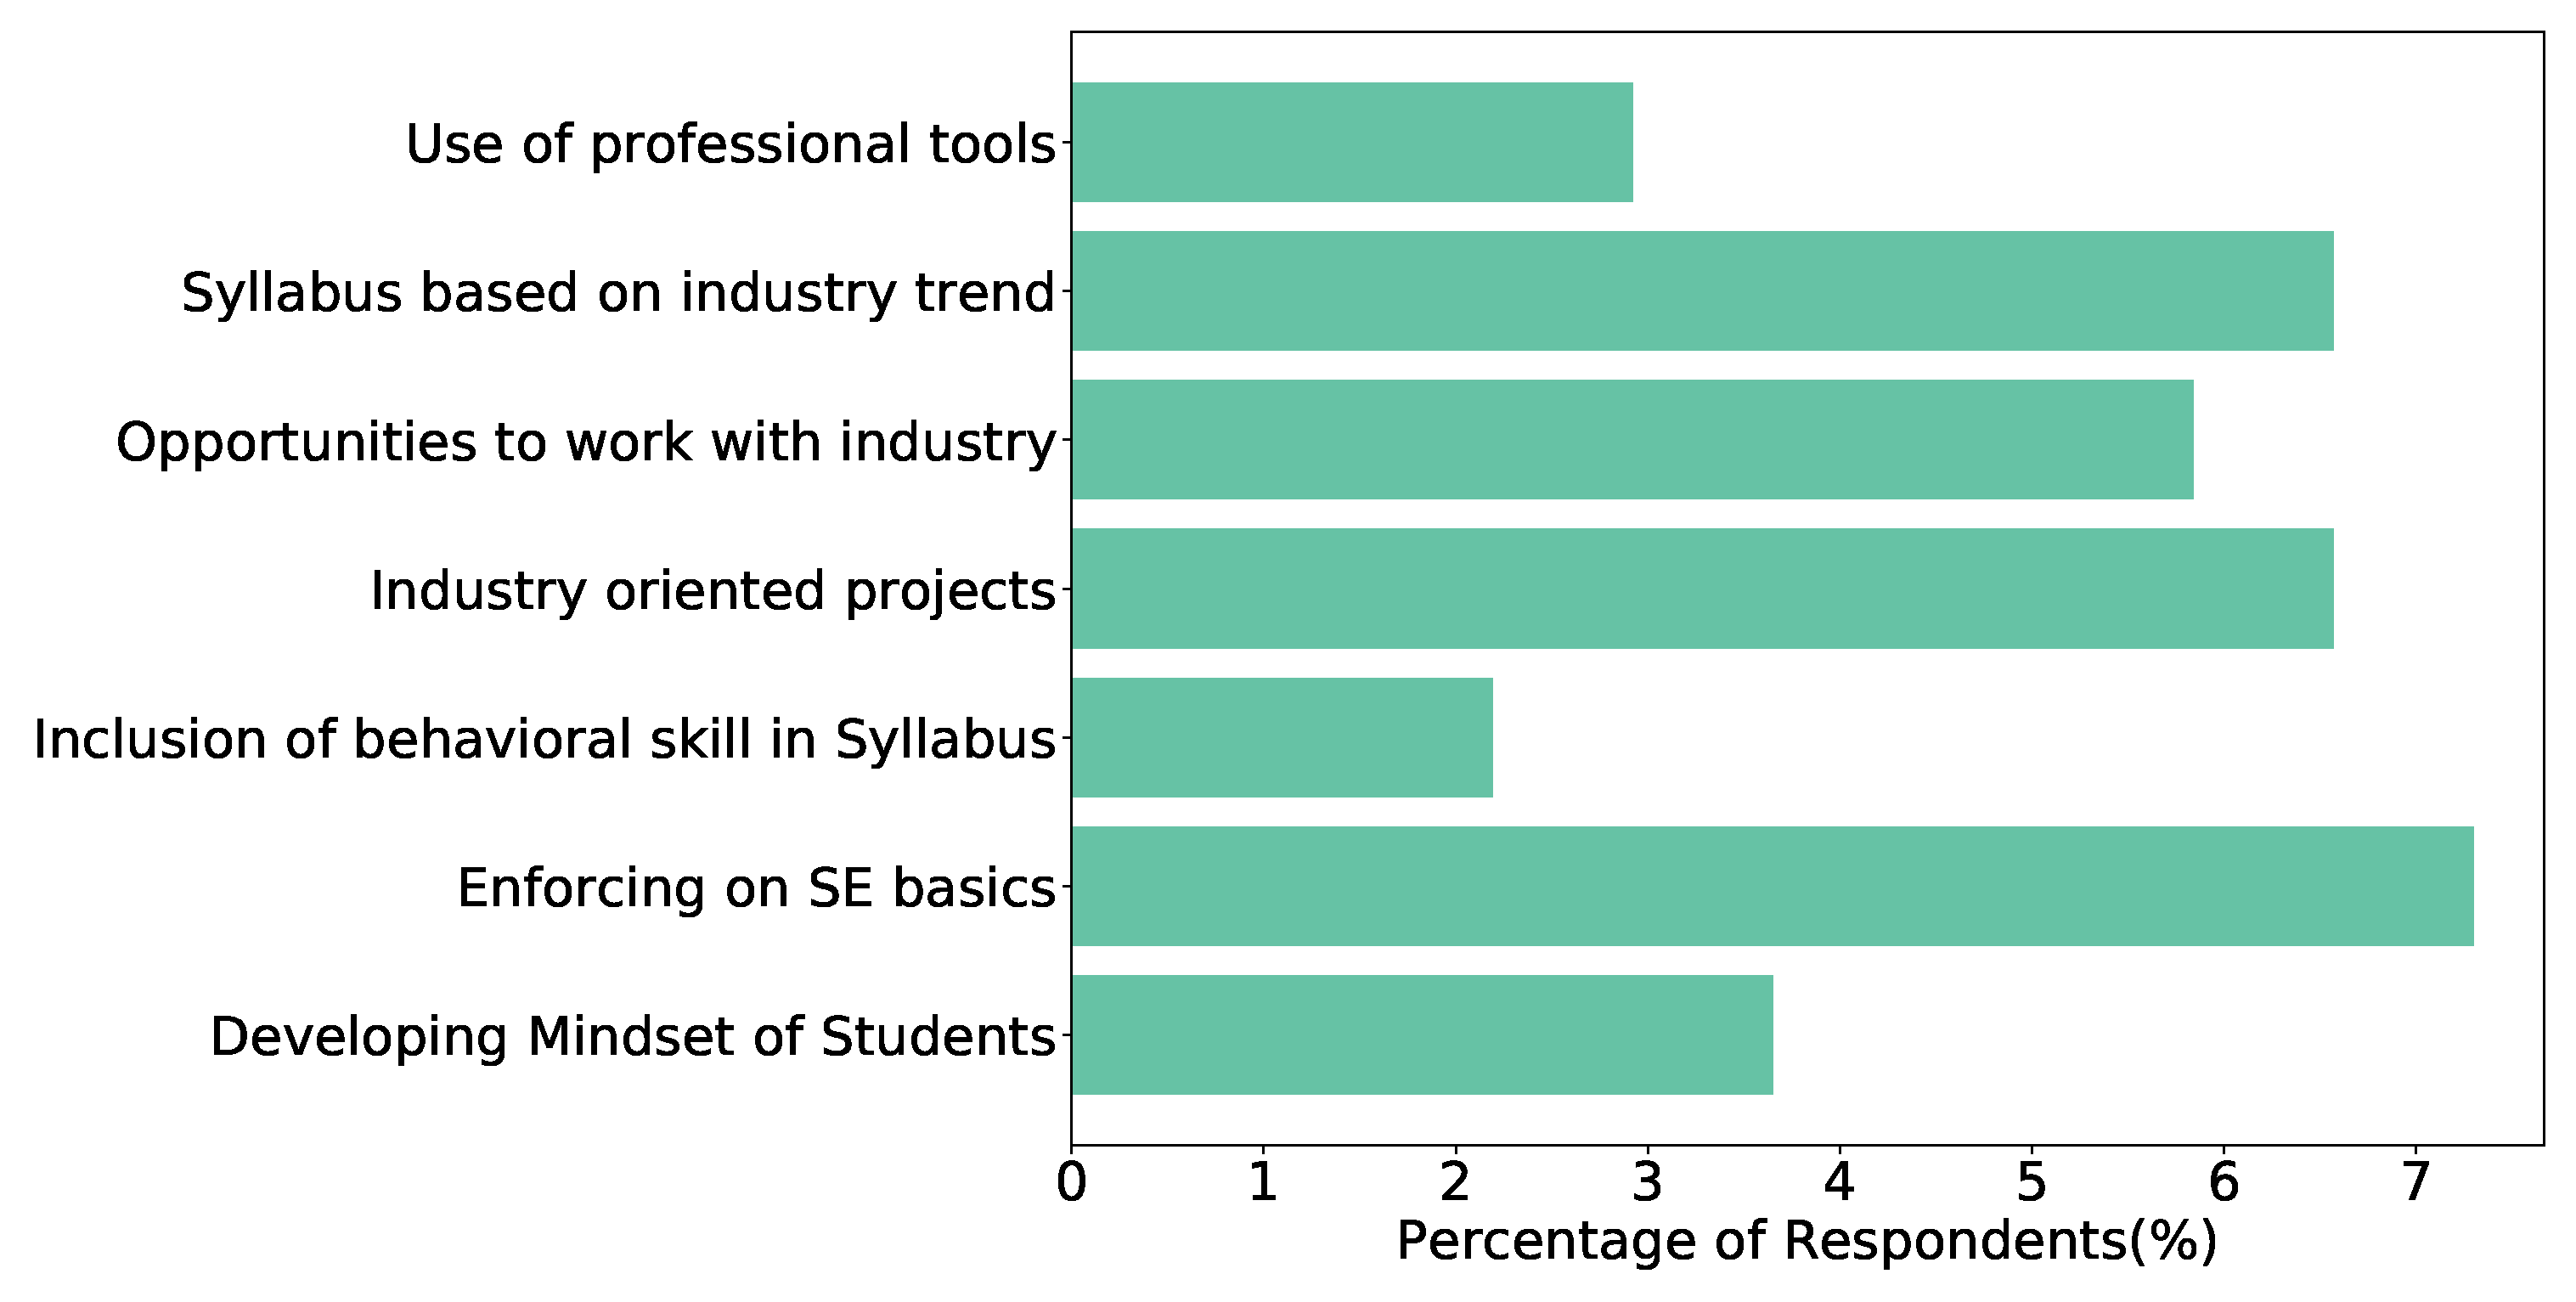
\includegraphics[scale=0.28]{Figures/UniversityExpectation.eps} 
\caption{Respondents expectation from university}
\label{fig:university expectation}
\end{figure}
\hfill\\
To have a vibrant SE industry and to maintain a steady workforce for the industry it is important that universities meet the expectation from the industry. As seen in Figure \ref{fig:university expectation}, industry owners/experts expect emphasis on SE basic and on current trends, they also seek for the opportunity to collaborate with the universities. The result coincides with  a study conducted by Radermacher et al. \cite{Radermacher2013}. According to their study, SE basic (Project Management, Software Tools, Testing) is the second area where graduate students are deficient in knowledge\cite{Radermacher2013}. Though behavioral skill or soft skill enables faster integration and happier teams only 2.19\% respondents emphasize on inclusion of behavioral skill in syllabus, the scenario is quite different in New Zealand. In a survey conducted by Stevens et al.\cite{Stevens2016} it is found that industry experts emphasize on behavioral skills after technical skill. They also found that those skills are un-trainable in work place. Thus it is the duty of university to train graduates with required skill set.
\begin{enumerate}
    
    
    \item \textbf{Inclusion of behavioral skill in Syllabus}: Being a good coder is difficult, but being a good human being is much more difficult. In industry, a person has to meet a large variety of personalities, and only a well behaved individual will find it easy to work with them. About 2.19\% people have implied about it.
    \surveyquote{Teach students Professional Ethics and Practices, Tie-up with Industry Practices and Problems, Solutions or Research Paper for any specific or generic Technical/Administrative problems}{108}
    
    
    
    \item \textbf{Syllabus based on industry trend}:It is seen in some universities in our country that they are teaching on a syllabus which was designed a very very long time ago. Since then software industry has advanced a long way. 6.57\% of our respondents think that these age-old academic curriculum should be changed and new latest topic should be added.
    \surveyquote{Concentrate on applied science with theory. Change syllabus based on current trend each year. Apply internship to relevant organisations}{5}
    
    
    
    \item \textbf{Opportunity to work with industry}:  As many students will be joining the industry after graduation, it will be very convenient for everyone if they are acquainted with the industry in their varsity life. 5.84\% respondents have felt the necessity of industry-academia correlation.
    \surveyquote{Create opportunities to work with industry solving the problems we are facing in the industry. Sometimes we are so busy with developing features that we lack the opportunity to run some researches about our tasks. University projects can be subjected to s...}{10}
    
    
    
    \item \textbf{Industry oriented projects}: 6.57\% respondents wants that in university student should engage in projects which is relevant to industry.
    \surveyquote{Connection with industry, realistic teaching, internship arrangement for students}{59}
    
    
    
    \item \textbf{Enforcing on SE basics}: 7.3\% respondents emphasized on SE  basics. They want prioritization of SE basic in university syllabus. The respondents mentioned design and delivery system, testing tools and design pattern in their response.
    \surveyquote{University should train student some basic knowledge of industry practice. Research on industry SDLC.}{115}
    
    
    
    \item \textbf{Developing mindset of students}: To have a keen interest to learn new technological knowledge is a must for every students. This mindset will not be developed in a day. They have to practise it for a long time. 3.65\% respondents feel that teachers as well as universities can help them to achieve it.
    \surveyquote{Develop mind set of student so that they love challenges, enjoy taking initiatives , never fear a problem and always ready to learn. It should teach students basic behavioral skills like honesty, integrity, accept failure and criticism positively , respect...}{35}
    
    
    
    \item \textbf{Use of professional tools}: 2.92\% respondents expects that university should make their student acquainted with professional software engineering tools like version controlling system, testing suits etc.
    \surveyquote{They should introduce students to version controlling. Code quality can be also an important thing}{57}
    
\end{enumerate}

\subsubsection{Expectation from Government}
\label{Expectation from Government}
\begin{figure}[htbp]
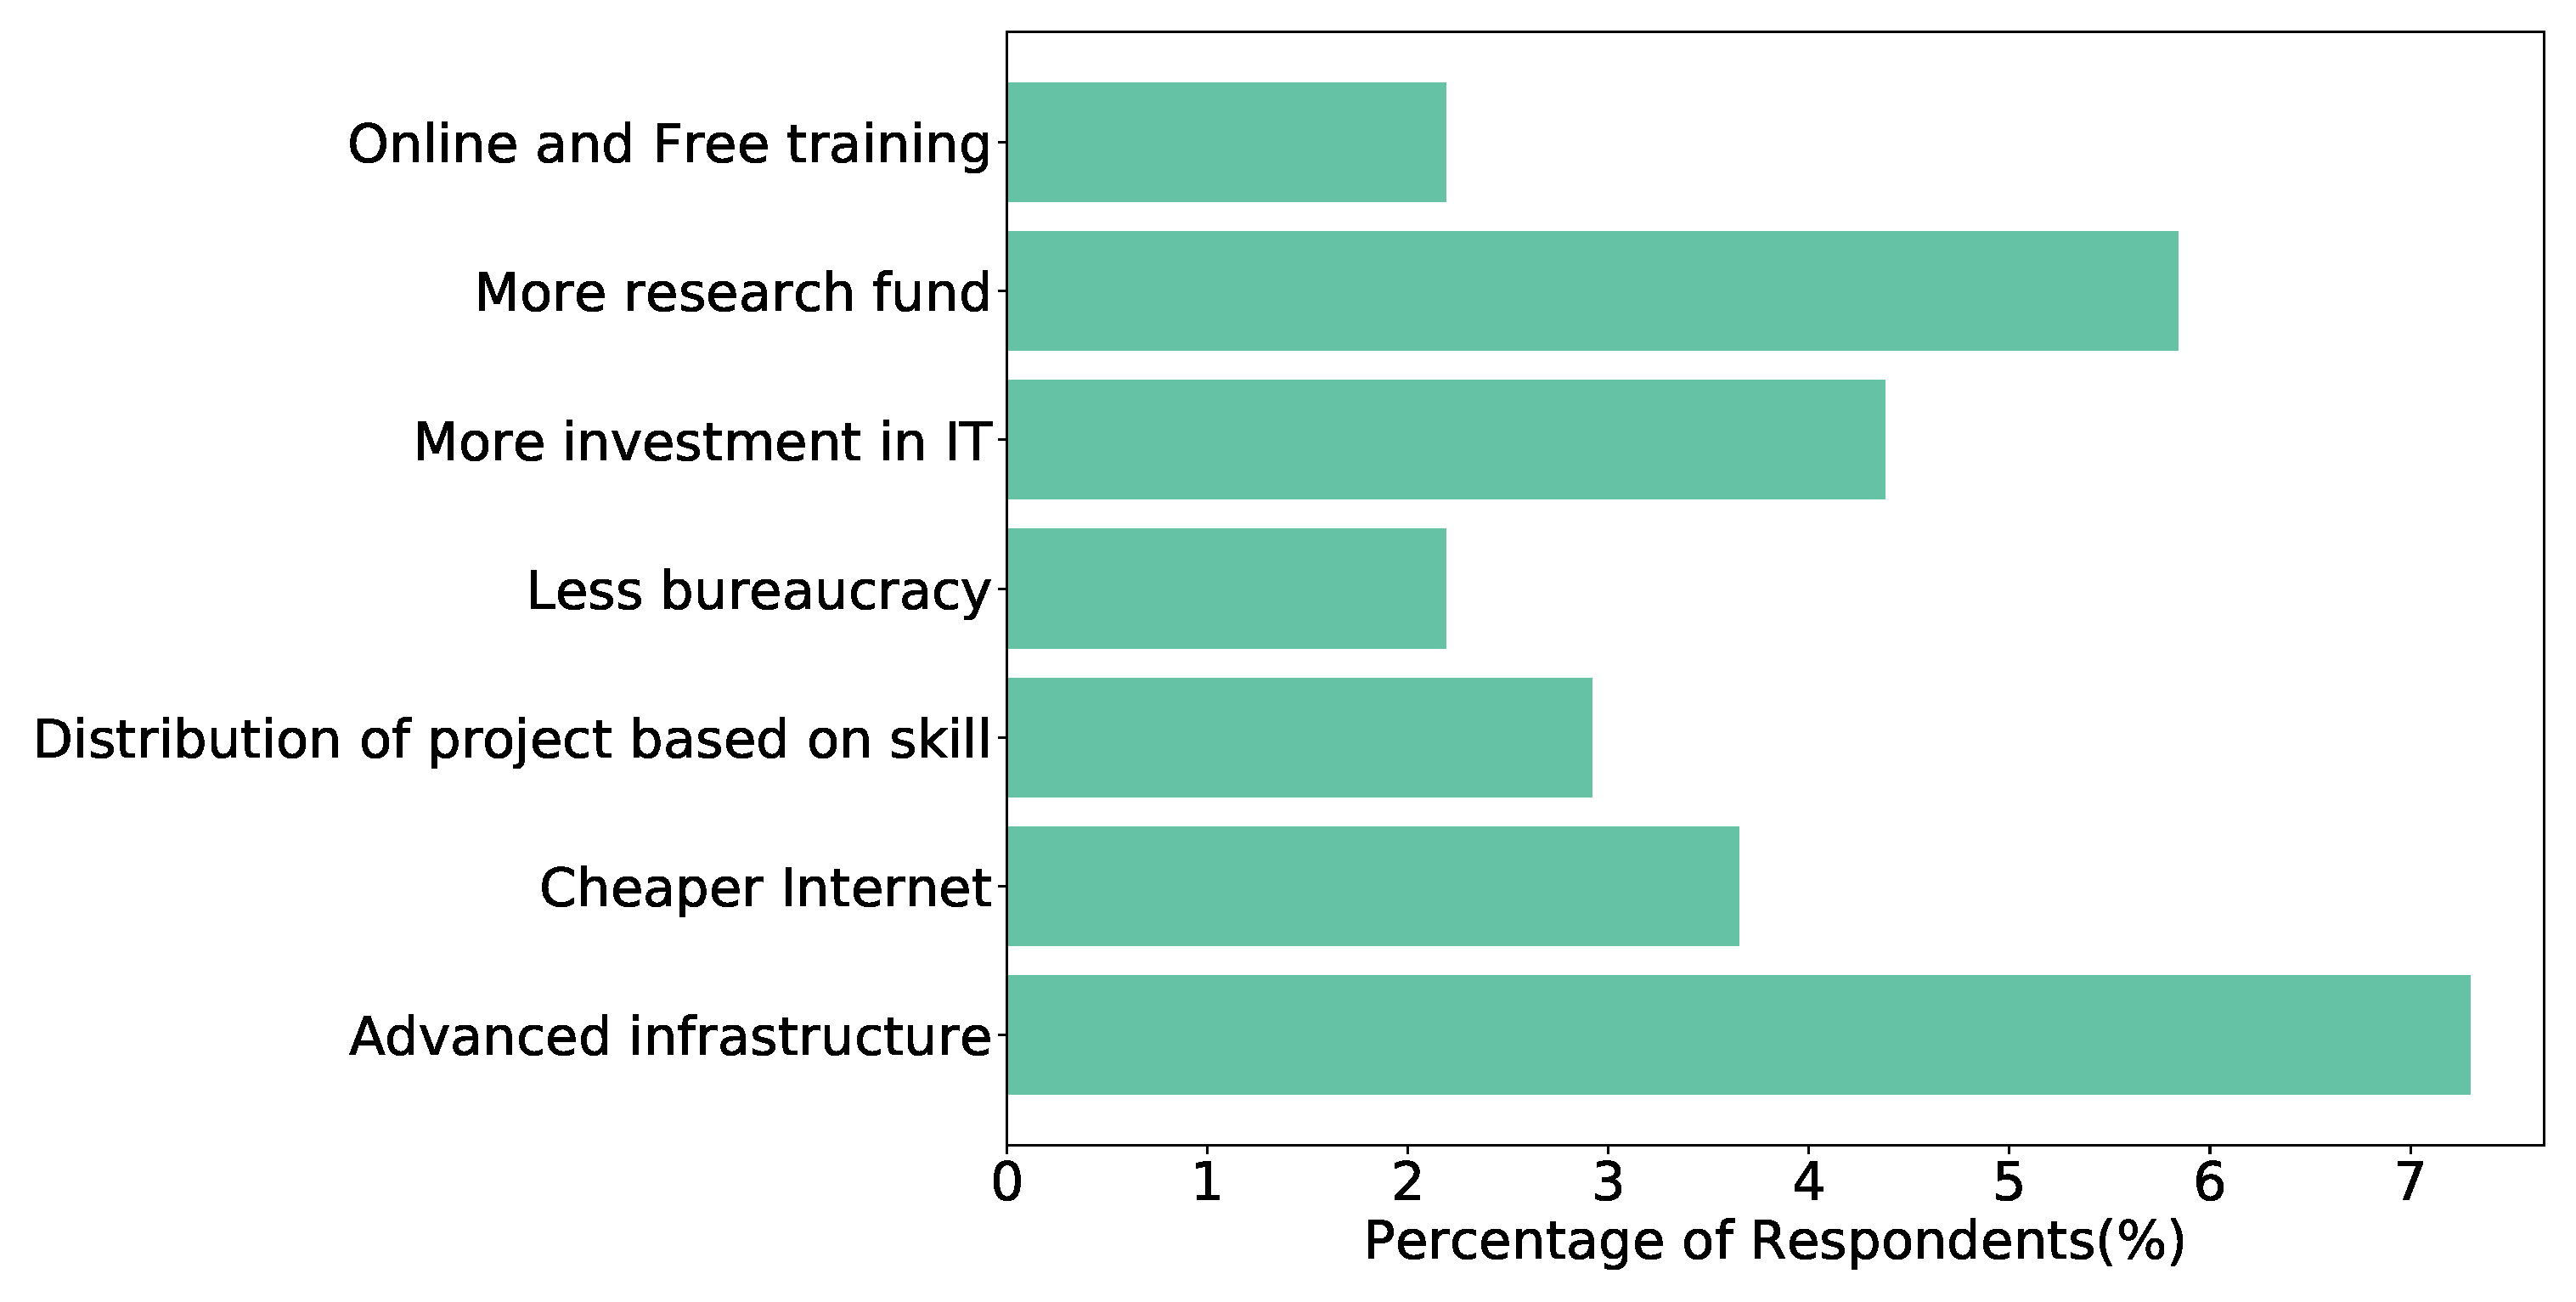
\includegraphics[scale=0.28]{Figures/GovernmentExpectation.eps} 
\caption{Respondents expectation from governmentt}
\label{fig:government expectation}
\end{figure}
\hfill\\
Government policies shapes the future SE industry. Tessler et al.\cite{Tessler2003} completed a study to rank the possible action for government for boosting the IT industry. They have ranked infrastructure and telecommunication as the first two action for government. The result is similar to our study where the 7.3\% respondents  expects  better infrastructure from government.
\begin{enumerate}
    \item \textbf{Online and free training}: If government arranges free and online training, the professionals can learn a lot more alongside with the private training. 2.19\% of our respondents have demanded for free online workshop.
    \surveyquote{1.online Free training center for easy learning it from Advance level (industry level) , Not basic level}{128}
    
    \item\textbf{More research fund}: In our country, research funds issued by government is really really less than expected. If we want to emerge as a country of developed software industry, government have to issue more money on research on this sector. 5.84\% respondents think that it is very hard to develop software industry with such little funds.
    \surveyquote{Issuing research funds to the universities to run researches. Government should emphasize in automation in every possible sector}{10}
    
    \item\textbf{More investment in IT}: 4.38\% respondents wants more investment  in IT sector from the govern met. Respondents mention steps like tax waiver and creating opportunities for domestic companies in government projects.
    \surveyquote{Tax benefits, infrastructure}{66}
    
    \item\textbf{Less bureaucracy}: 2.19\% of respondents want the removal of red tape from the administrative process as it prevents the development of the IT industry.
    \surveyquote{get yourself out of corruption. and let yourself put in liability}{133}
    
    \item\textbf{Distribution of project based on skill}: It is frequently seen in our country that less expert and less eligible persons are getting priority than more eligible persons because of nepotism. 2.92\% of our respondents think that it should be eliminated as soon as possible for the sake of industry development.
    \surveyquote{Proper maintenance with previous projects and follow up. Plan next years with long vision through solid IT-specialists. Distribute projects based on skills than links. Remove bureaucratic process for small companies to contribute more for country}{5}
    
    \item\textbf{Cheaper internet}: In this age, it is difficult to spend a single day without internet. As it is also a great source of learning as well as earning, government should remove tax from internet charge and give internet in exchange of a very lower rate. Some people have also asked for 5G.
    \surveyquote{faster and cheaper internet infrastructure}{74}
    
    \item\textbf{Advanced infrastructure}: 7.3\% respondents expects advanced infrastructure like IT/software parks, data center from government.
    \surveyquote{Improved transport system, Software development zone with competitive rent}{85}
    
\end{enumerate}

\subsubsection{Training provide by Companies}
\label{Training provide by Companies}
\begin{figure}[htbp]
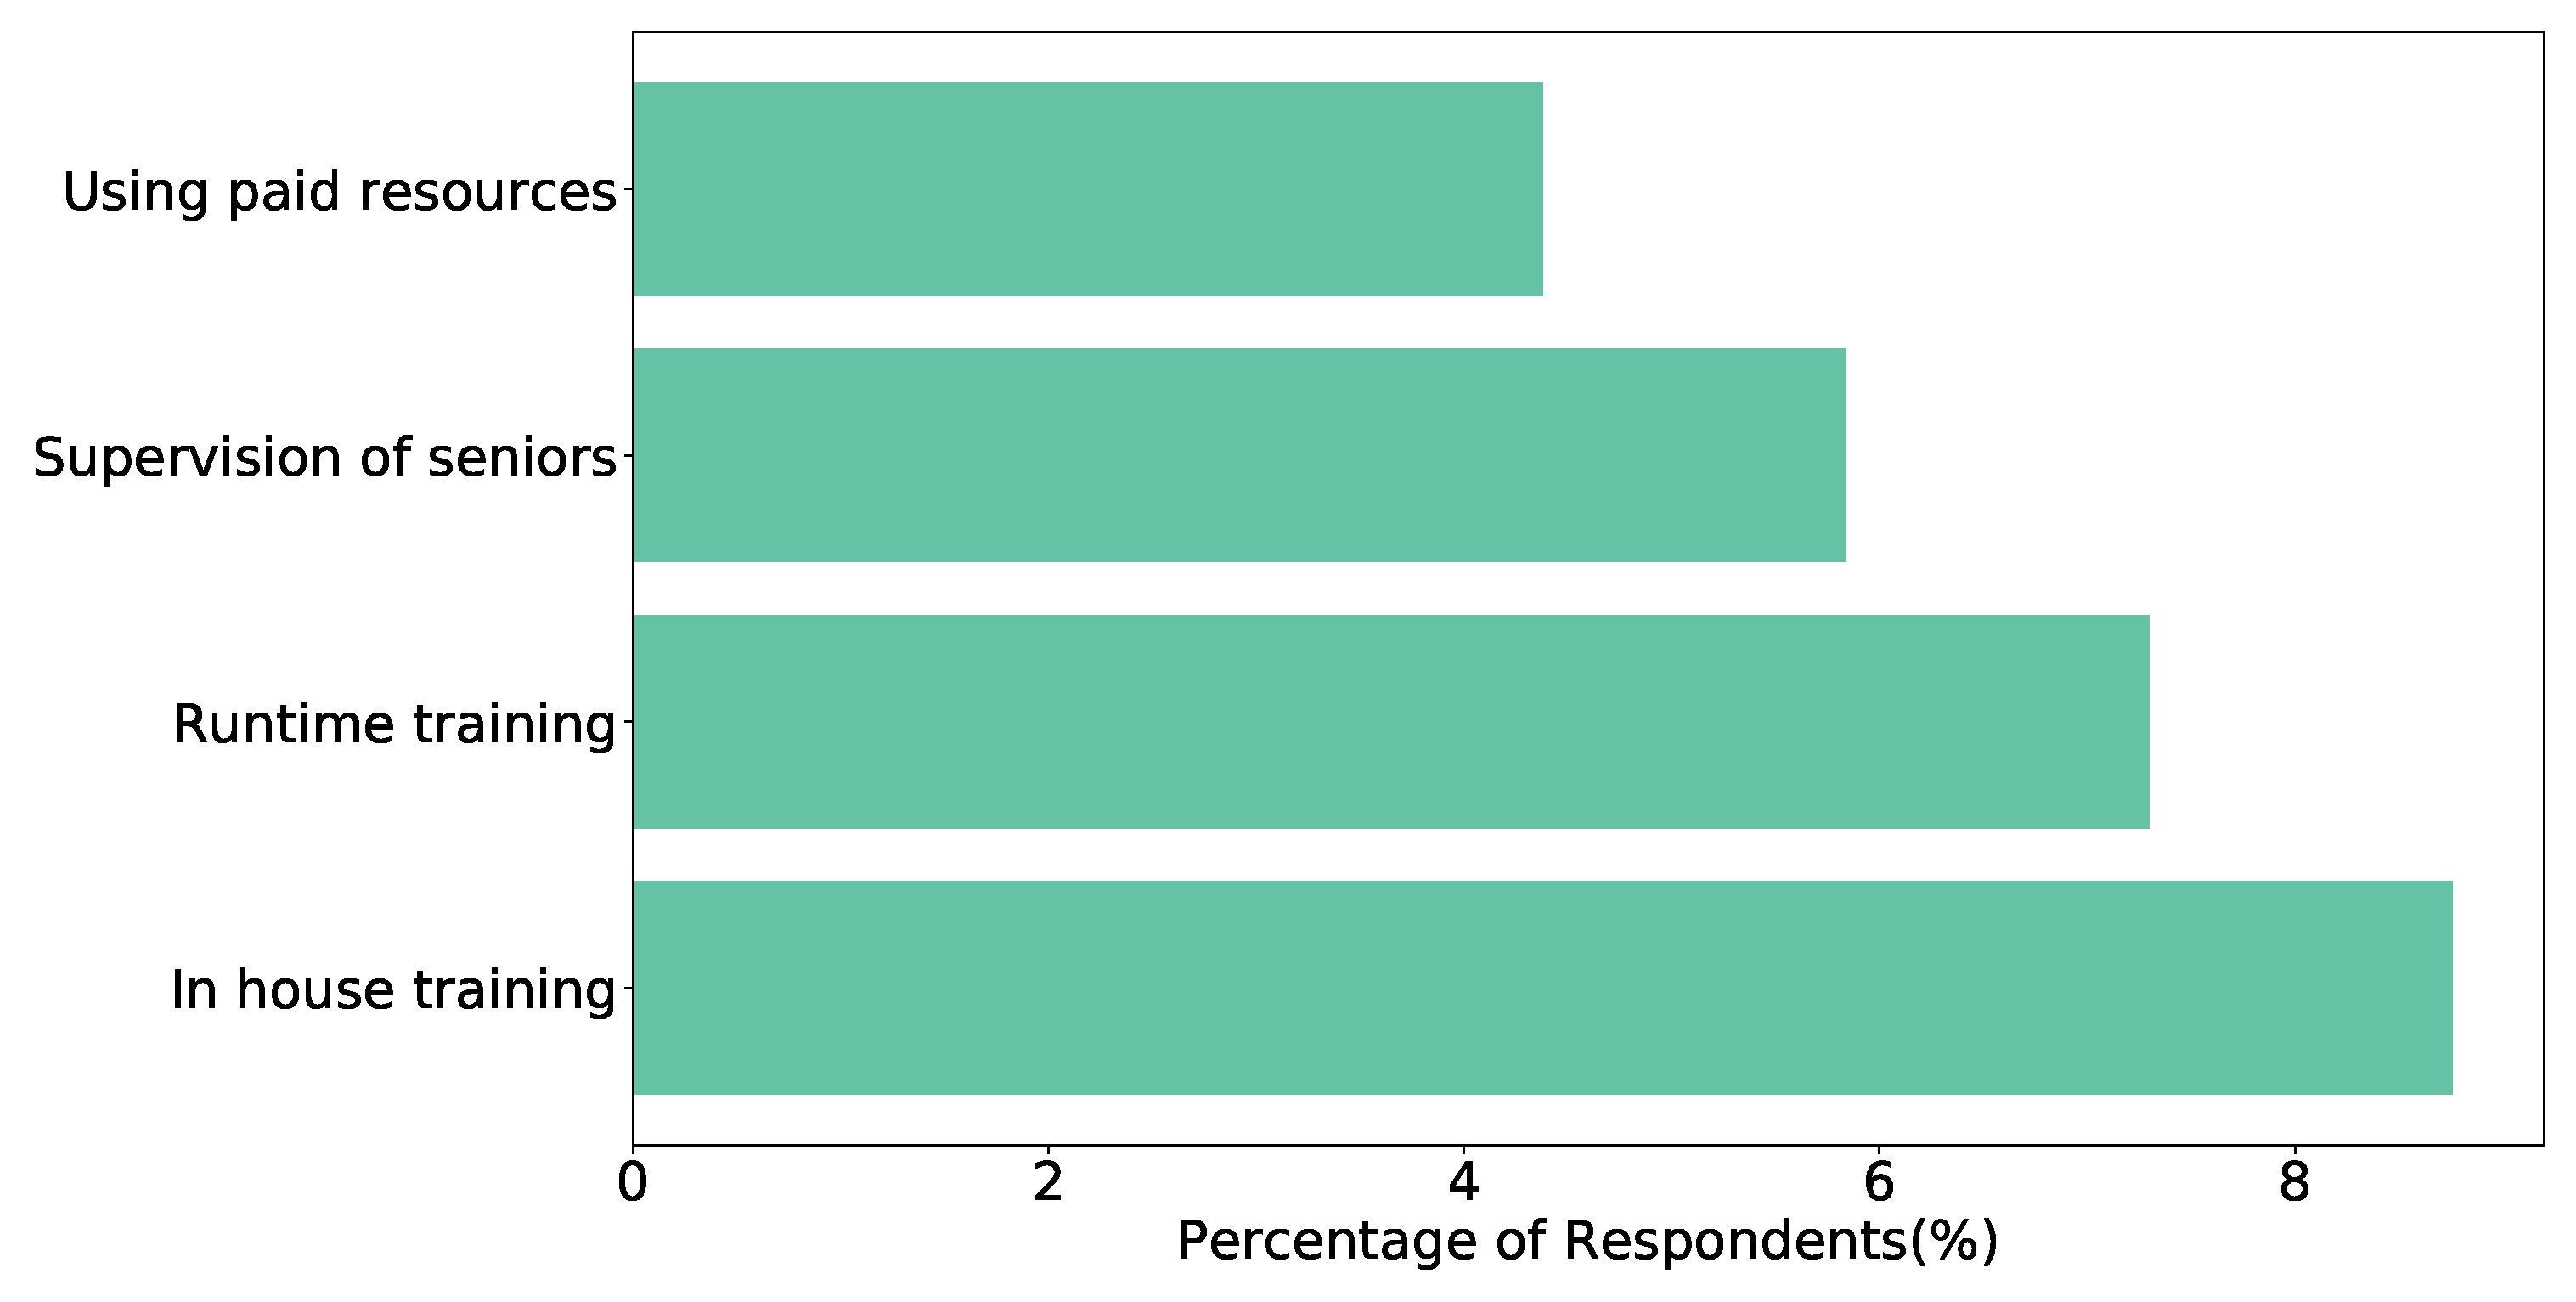
\includegraphics[scale=0.28]{Figures/Training.eps} 
\caption{Respondents expectation from government}
\label{fig:company training}
\end{figure}
\hfill\\
In order to adapt to the new technologies and drive new employees, staff training sessions are required in SE firms. From the survey, it is clear that in house training is the most popular form of training in the SE industry in Bangladesh. In the Australian \cite{Ng2004} and Hong Kong\cite{Chan2005} SE industry , the scenario is different where the most popular form of training is commercial courses and then in house training.  The difference in popularity can be linked to economic conditions. As the SE industry of Bangladesh is not mature, it is clear that SE companies will not be able to spend money on paid training courses.

\begin{enumerate}
    \item \textbf{Using paid resources}: 4.38\% respondents mentioned that they use online paid resources or certification courses to train their employees.
    \surveyquote{We have pluralsight account and we perform bimonthly technical session}{57}
    
    \item\textbf{Supervision of seniors}: Being supervised by the seniors is the best way of training. They can teach us from their experience and experience teaches a lot.
    \surveyquote{mentoring}{74}
    
    \item\textbf{Runtime training}: About 7.3\% people have said that they provide their employees with runtime training.
    \surveyquote{Run time training through small scale project and supervision of seniors}{5}
    
    \item\textbf{In house training}: Companies also provide their employees with tutorials and books so that they can read at their home and get used to the practices followed.
    \surveyquote{Internal knowledge sharing sessions}{53}
    
\end{enumerate}


